\chapter{Kontrollieren}\label{ch:kontrollieren}
Dieses Kapitel zeigt die in der IPERKA-Phase «Kontrollieren» durchgeführten Arbeiten auf. In dieser Phase wird beschrieben, wie der Lernende die Tests implementiert hat und welche Technologien schlussendlich verwendet wurden.

\section{Allgemein}
Die Tests wurden im entsprechenden Ordner «test» erstellt. In diesem Ordner existieren auch bereits andere Tests und auch Unterkategorien wie configuration, integrationtest, resource, shared und util. Die geplanten Tests wurden in dem Ordner integrationtest und resource erstellt und implementiert. Um die Tests zu schreiben und mit @Test zu deklarieren wurde JUnit \footnote{\url{https://junit.org/junit5/}} verwendet.

\section{Integration-Tests}
Für die Erstellung der Daten wurde eine interne Klasse des CardX-Projekts verwendet. Die Klasse trägt den Namen «A» und ermöglicht es von vielen PCs im Projekt, ein Objekt zu erstellen, welches anschliessend in einer Datenbank gespeichert wird und das erstellte Objekt zurückgibt. Diese Klasse wurde verwendet, um verschiedene MqTablePC-Objekte zu erstellen und sie daraufhin für die Endpoints zu nutzen.

\subsection{testGetAllMqIns}
Dieser Test überprüft die Funktionalität des GET-Request, um alle MqIns mit dem Status ERROR hervorzuholen. Die Objekte werden mithilfe von einer erstellten Funktion erstellt und anschliessend ein GET-Request auf den zu testenden Endoint gemacht. Dieser Request wird mit WebCliend gemacht, der von dem Springframework zur verfügung gestellt wird.

\begin{verbatim}
	MqInDto[] mqInDtos = WebClient.create("http://localhost:" + getPort())
	.get()
	.uri(PATH)
	.retrieve()
	.bodyToMono(MqInDto[].class)
	.block();
\end{verbatim}

\paragraph{.get()} deklariert den Request als GET-Request.
\paragraph{.uri(PATH)} wird verwendet, um den Pfad des Endpoints anzugeben.
\paragraph{.retrieve()} wird im Zusammenhang mit bodyToMono() verwendet.
\paragraph{.bodyToMono(MqInDto[].class)} stellt sicher, dass der Rückgabewert eine Liste von MqInDtos ist.
\paragraph{.block()} blockiert alle synchronen Requests bis dieser Request abgeschlossen ist.

Das Resultat des Requests wurde anschliessend mit «assertNotNull» und «asserThat» überprüft auf Richtigkeit. Zuerst wurde geschaut, ob die erhaltene Liste null ist und anschliessend die Länge und den Inhalt auf Korrektheit geprüft.

\subsection{testExecuteNewProcessingAttempt}
Das Verfahren der Implementierung dieses Tests ist fast gleich. Der Unterschied ist, dass zweimal ein Get-Request ausgeführt wird. Das erste Mal, um den ursprünglichen Stand der Datenbank hervorzuholen und ein zweites Mal, nach dem der PUT-Request getätigt wurde, um zu überprüfen, ob das Objekt überschrieben wurde. 

Der PUT-Request ist gleich aufgebaut wie die GET-Requests, mit zwei kleinen Unterschieden. Es wurde ein Body hinzugefügt, mit der id des zu überschreibenden Objekts, und das .get() wurde mit .put() ersetzt. 

\begin{verbatim}
	Long idOfMqIn = Arrays.stream(mqInsBevorUpdate).findFirst().get().getId();
	Integer response = WebClient.create("http://localhost:" + getPort())
	.put()
	.uri(PATH + "/")
	.body(Mono.just(idOfMqIn), Long.class)
	.retrieve()
	.bodyToMono(Integer.class)
	.block();
\end{verbatim}

\subsection{testGetFilteredMqInEntries}
Für das Testen der Filter-Requests wurde ein MqInFilterDto Objekt erstellt und mit den folgenden Filtern befüllt:

\begin{itemize}
	\item Nachricht: mqTable3
	\item Status: NEW
	\item Datum bis: 202.11.20TT23:00:00
\end{itemize}

Das Filterergebnis sollte alles herausfiltern, bis auf ein Element. Dieses wurde anschliessend auf die Richtigkeit des Status, der Nachricht und dem Datum bis.

\begin{verbatim}
	@Test
	void testGetFilteredMqInEntries() {
		setupDB();
		
		MqInFilterDto filter = new MqInFilterDto();
		filter.setMessageQuery("mqTable3");
		filter.setStatus("NEW");
		filter.setTimestampTo(LocalDateTime.of(2024, 11, 20, 23, 0, 0).toString());
		
		MqInDto[] mqIns = WebClient.create("http://localhost:" + getPort())
		.put()
		.uri(PATH + "/filtered")
		.body(Mono.just(filter), MqInFilterDto.class)
		.retrieve()
		.bodyToMono(MqInDto[].class)
		.block();
		
		assertNotNull(mqIns);
		assertThat(mqIns.length).isEqualTo(1);
		assertThat(mqIns[0].getMqInStatus()).isEqualTo(MqInStatus.NEW);
		assertThat(mqIns[0].getMessage()).isEqualTo("mqTable3");
	}
\end{verbatim}

\section{Unit-Tests}
Um die Daten für das Testing bereitzustellen, wurde eine Klasse MqInMock erstellt. Diese Klasse beinhaltet ein paar Funktionen, welche ein, mehrere oder verschiedene MqTablePCs zurückgibt.

\subsection{testMappingWithSinglePC}
Dieser Test überprüft die Funktion toMqInDto(MqTablePC mqTablePC), welche aus einem MqTablePC-Objekt ein MqInDto-Objekt mappt. Der Test selbst ist einfach aufgebaut. Er erstellt zuerst das zu mappende Objekt und gibt es anschliessend als Parameter beim Aufruf der Funktion mit. Danach wird mithilfe von assertNotNull() und assertThat() überprüft, ob es existiert und ob alle Werte richtig gesetzt wurden.

\subsection{testMappingWithMultiplePCs}
Hier wird ein ähnlicher Ablauf verwendet wie beim Test zuvor. Der Unterschied liegt aber dabei, dass die Funktion listToMqInDto(List<MqTablePc> listOfMqTablePCs) aufgerufen wird und eine Liste mitgegeben wird. Bei der Überprüfung wird ausserdem durch die erhaltene Liste iteriert und bei jedem einzelnen Element die erwarteten Werte überprüft.

\begin{verbatim}
	@Test
	void testMappingWithMultiplePCs() {
		// given
		List<MqTablePC> mqTablePCs = MqInMocks.createEveryStatusTypeOfMqTablePC();
		
		// when
		List<MqInDto> mqInDtos = mapper.listToMqInDto(mqTablePCs);
		
		// then
		assertNotNull(mqInDtos);
		for (MqTablePC mqTablePC : mqTablePCs) {
			MqInDto mqInDto = mqInDtos.stream().filter(mqIn -> mqIn.getId() == mqTablePC.getId()).findFirst().get();
			assertNotNull(mqInDto);
			assertThat(mqInDto.getId()).isEqualTo(mqTablePC.getId());
			assertThat(mqInDto.getMessage()).isEqualTo(mqTablePC.getMessage());
			assertThat(mqInDto.getJobKey()).isEqualTo(mqTablePC.getJobKey());
			assertThat(mqInDto.getModifiedAt()).isEqualTo(mqTablePC.getModifiedAt());
			assertThat(mqInDto.getMqQueueId()).isEqualTo(mqTablePC.getMqQueueId());
			assertThat(mqInDto.getProcessedCnt()).isEqualTo(mqTablePC.getProcessedCnt());
			assertThat(mqInDto.getMqInStatusString()).isEqualTo(mqTablePC.getMqInStatusString());
			assertThat(mqInDto.getMqInStatus()).isEqualTo(mqTablePC.getMqInStatus());
		}
	}
\end{verbatim}

\subsection{testMappingOfMqInFilterDto}
Dieser Test ist gleich aufgebaut wie der erste Test. Die verwendeten Klassen sind anders. Vom gröberen Aufbau ist es aber der gleiche Test, einfach für eine andere Funktion. Er überprüft die Funktionalität der toMqTableFilterQuery Funktion für den Filter der Elemente.

\begin{verbatim}
	@Test
	void testMappingOfMqInFilterDto() {
		// given
		MqInFilterDto filterDto = MqInMocks.createMqInFilterDto();
		
		// when
		MqTableDao.MqTableFilterQuery result = mapper.toMqTableFilterQuery(filterDto);
		
		// then
		assertNotNull(result);
		assertThat(result.status()).isEqualTo(MqInStatus.ERROR);
		assertThat(result.messageQuery()).isEqualTo("mqTable1");
		assertThat(result.timestampFrom()).isEqualTo(OffsetDateTime.of(2024, 11, 20, 10, 0, 0, 0, ZoneOffset.ofHours(1)));
		assertThat(result.timestampTo()).isEqualTo(OffsetDateTime.of(2024, 11, 20, 20, 0, 0, 0, ZoneOffset.ofHours(1)));
	}
\end{verbatim}

\section{Codequalität prüfen}
Für die Überprüfung der Codequalität wird das integrierte Jenkins im Projekt CardX verwendet.

\subsection{Verlauf der Prüfung von der Codequalität}

\begin{figure}[H]
	\begin{center}
		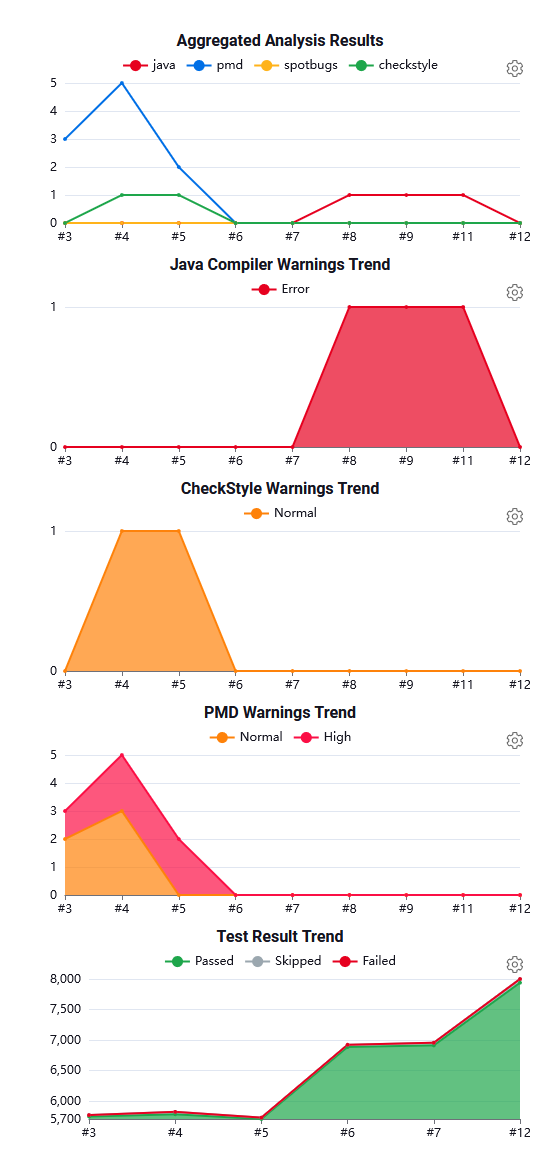
\includegraphics[width=0.6\textwidth]{ressourcen/Build-verlauf}
		\caption[Codequalität Verlauf]{Codequalität Verlauf}\label{ch:build-verlauf}
	\end{center}
\end{figure}

Die Abbildung \ref{ch:build-verlauf} zeigt auf, warum die Builds fehlgeschlagen sind. Die dargestellten Graphen werden hier kurz erklärt, um einen besseren Überblick zu verschaffen.

\paragraph{Aggregated Analysis Result} zeigt von jedem Build an, welche Codequalitäten-Checks fehlgeschlagen oder nicht erfüllt wurden.
\paragraph{Java Compiler Warnings Trend} zeigt an, ob beim compilieren des Java-Codes ein Fehler auftrat.
\paragraph{Checkstyle Warnings Trend} zeigt auf, wie viele Ceckstyles nicht erfüllt wurden. Checkstyles stellen sicher, dass der Code sauber, lesbar und einheitlich bleibt.
\paragraph{PMD Warnings Trend} zeigt auf, wie viele Warnungen der Code aufweist. PMD wird verwendet, um den Code auf potenzielle Probleme zu untersuchen, ohne den Code auszuführen.\newline

\noindent Der letzte Build \#12 zeigt, dass alle Tests, CodeQualitäten und Warnungen gelöst wurden und ist durch das grün.

\subsection{Falscher Rückgabewert bei setMqInStatusToNew}
Die Funktion setMqInStatusToNew() hatte von den PMD-Warnungen aus einen falschen Rückgabewert (int). Diese Warnung tauchte auf wegen des Namens. Da ein «set» im Namen vorhanden war, wurde vermutet, dass es ein Setter ist, was aber nicht der Fall war. Die Funktion wurde daraufhin umbenannt zu executeNewProcessingAttempt(), was das Problem löste.

\subsection{JUnit-Test Klassen müssen final sein}
Um die Sichtbarkeit der Testklassen einzuschränken, müssen diese Package-Private sein. Aus diesem Grund wurde die Sichtbarkeit von MqInIntegrationTest angepasst.

\subsection{LocalDateTime / -Millis.class}
Bei der Erstellung von den Mock-Daten in der Klasse MqInServiceMockImpl wurde der Datums-Typ LocalDateTime verwendet. Die Nutzung von diesem Typ wurde abgeraten und empfohlen, den Typ LocalDateTimeMillis zu nehmen, da hier die Millisekunden auch angezeigt werden.

\subsection{MqInMocks}
Die Klasse MqInMocks hat einen privaten Konstruktor und sollte in diesem Fall selbst eine «final» Klasse sein.

\newpage